\documentclass[pdf]{beamer}
\mode<presentation>{\usetheme{Boadilla}}
\usepackage{ragged2e}
\usepackage{etoolbox}
\usepackage{lipsum}
\usepackage{graphicx}


\graphicspath{ {./figure/} }
\apptocmd{\frame}{}{\justifying}{}

\newcommand{\N}{\mathbb{N}}
\newcommand{\Z}{\mathbb{Z}}
\newcommand{\Q}{\mathbb{Q}}
\newcommand{\R}{\mathbb{R}}
\newcommand{\C}{\mathbb{C}}
\newcommand{\hp}{\mathbb{H}}

%List of packages
%\usepackage{amsmath}

%%%%%%%%%%%%%%%%%%%%%%%%%%%%%% Metadata %%%%%%%%%%%%%%%%%%%%%%%%%%%%%%
\hypersetup
{
	%Separate multiple authors by comma
	pdfauthor={Yizi Wang},
	pdftitle={},
	pdfsubject={Instructions, Tutorials, Guidelines},
	pdfkeywords={SPSAS19, guidelines, presentation format},
	colorlinks=false
}

%%%%%%%%%%%%%%%%%%%%%%%%%%%%%% Title related %%%%%%%%%%%%%%%%%%%%%%%%%%%%%%
\setbeamertemplate{subsection in toc}[default]

%The contact for one of the authors MUST be embedded on the title (see below)
\title[Convergence Theories of the MCF]{Convergence Theories of\\ the Mean Curvature Flow}
%Subtitle (if needed)
\subtitle{}
%For LICENSE, we suggest CC-BY-SA, but you are free to choose your own as long
%as the LICENSE you choose is AT LEAST as permissive as CC-BY-SA
\date[2021]{June 10, 2021}
\author[WANG, Yizi]{\texorpdfstring{\textbf{WANG, Yizi}\\Thesis Defense Presentation\\Supervisor: Professor LI Man Chun}{WANG, Yizi}}
\institute[CUHK]{Department of Mathematics\\The Chinese University of Hong Kong}


%%%%%%%%%%%%%%%%%%%%%%%%% Presentation begins here %%%%%%%%%%%%%%%%%%%%%%%%%
\begin{document}

\begin{frame}
	\titlepage
\end{frame}


    \begin{frame}
        \frametitle{Mean Curvature Flow}
        \begin{definition}
            \justifying
            We say a family of hypersurfaces $\left\{ \Sigma_t \right\}$ in $\R^n$ satisfies the \textbf{Mean Curvature Flow} if they are evolving by the MCF equation \[\frac{\partial \vec{x}}{\partial t} =\vec{H}:=-H \vec{n}\] where $H$ is the mean curvature and $\vec{n}$ is the unit normal of $\Sigma_t$ at $\vec{x}$.
        \end{definition}
        
        \begin{figure}[h]
            \centering
            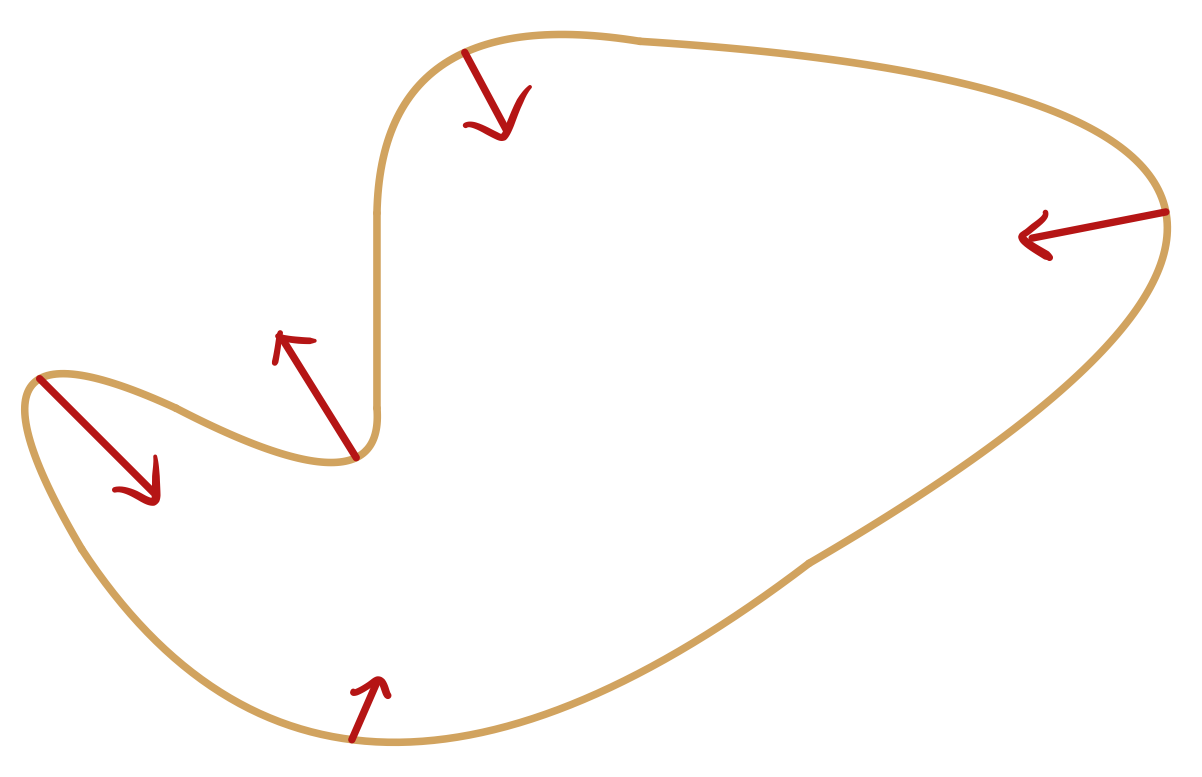
\includegraphics[scale=0.15]{MCF.png}
            \caption{A surface with mean curvature vector}
        \end{figure}
    \end{frame}

    \begin{frame}
        \frametitle{Mean Curvature Flow with Free Boundary}
        \begin{definition}
            \justifying
            Let $S \subset \R^{n+1}$  be a smooth embedded hypersurface without boundary with unit normal $\nu_S$. A hypersurface $\Sigma \subset \R^{n+1}$ is a \textbf{free boundary hypersurface} w.r.t. the ``barrier'' $S$ if \[\partial \Sigma  \subset S \text{ and }N = \nu _S\] where $N$ is the outward unit normal of $\partial \Sigma \subset \Sigma $.
        \end{definition}
        A family $\left\{ \Sigma_t \right\} $ of free boundary hypersurfaces satisfies \textbf{MCF with free boundary} if they satisfy the MCF equation in the interior.
        \begin{figure}[h]
            \centering
            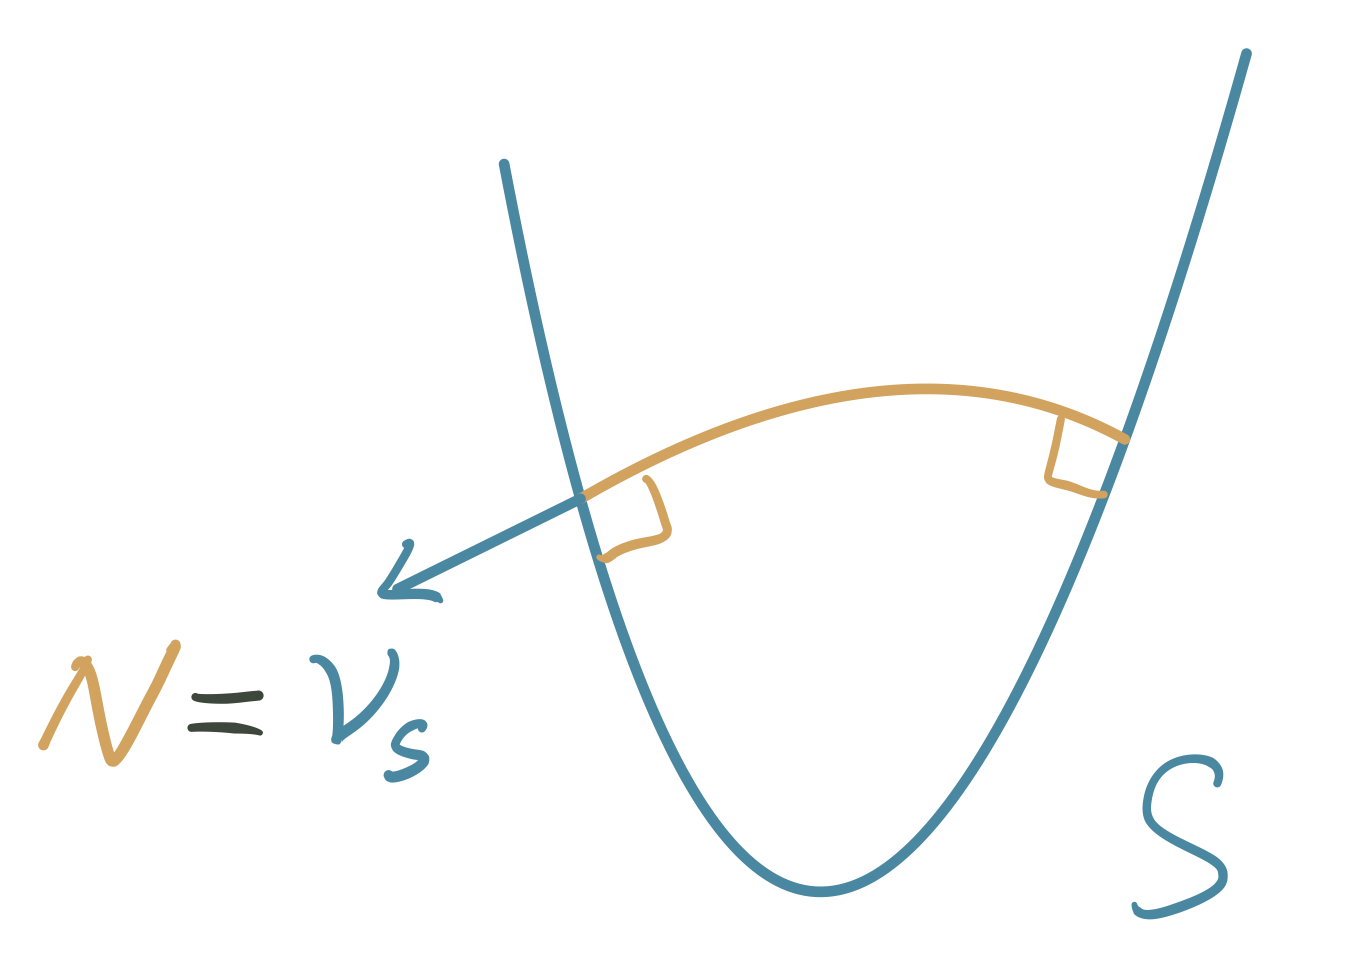
\includegraphics[scale=0.07]{FrBdy.png}
            \caption{A surface with free boundary on $S$}
        \end{figure}
    \end{frame}

    \begin{frame}
        \frametitle{Convergence of Mean Curvature Flow}

        \begin{columns}[T]
                \begin{column}{.65\textwidth}
                    \begin{theorem}[Huisken(1984), Gage-Hamilton (1986), Grayson (1987)]
                        \justifying
                        Any compact, convex hypersurface in $\R^n$ converges to a round point under MCF.
                    \end{theorem}
                    Generalized to Riemannian submanifolds by \textbf{Huisken(1986)}, \textbf{Grayson(1989)}.
                \end{column}
                \begin{column}{.35\textwidth}
                
            \begin{figure}[h]
                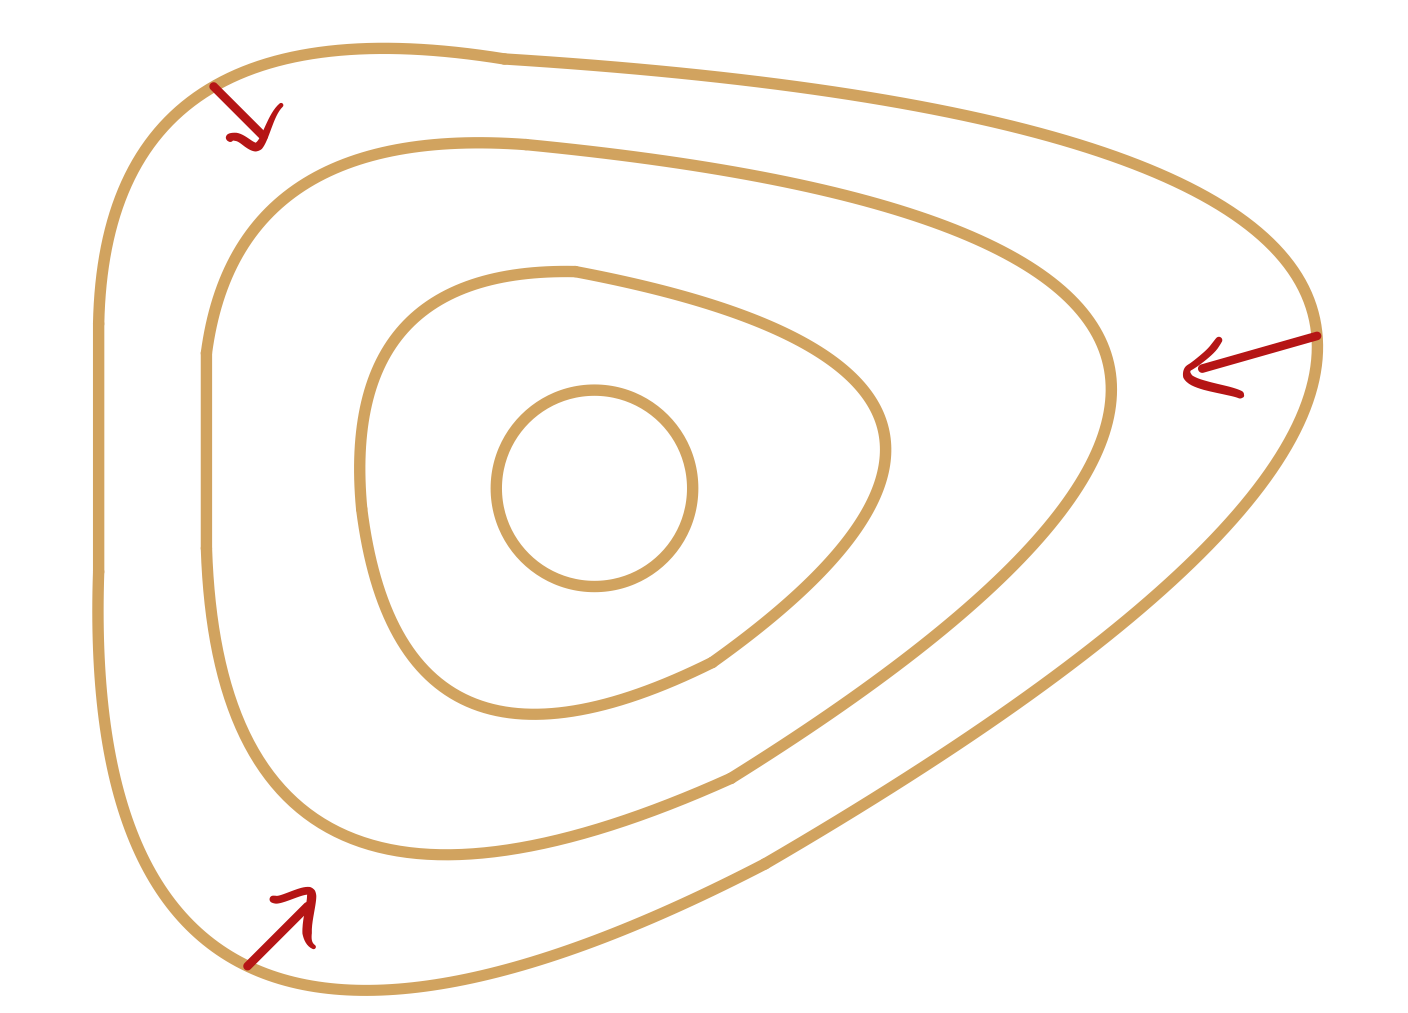
\includegraphics[scale=0.1]{HuCon.png}
            \end{figure}
            
                
                \end{column}
            \end{columns}
            \vspace{0.6cm}
            \begin{columns}[T]
                \begin{column}{.65\textwidth}
                    \begin{theorem}[(Stahl(1996), Edelen(2016)]
                        \justifying
                        Any compact, convex hypersurface in $\R^n$ with free boundary on a \textcolor{red}{sphere} converges to a round \textcolor{red}{half-point} under MCF.
                    \end{theorem}
                    Generalized to general convex barriers by \textbf{Hirsch-Li(2020)}.
                \end{column}
                \begin{column}{.35\textwidth}
                
            \begin{figure}[h]
                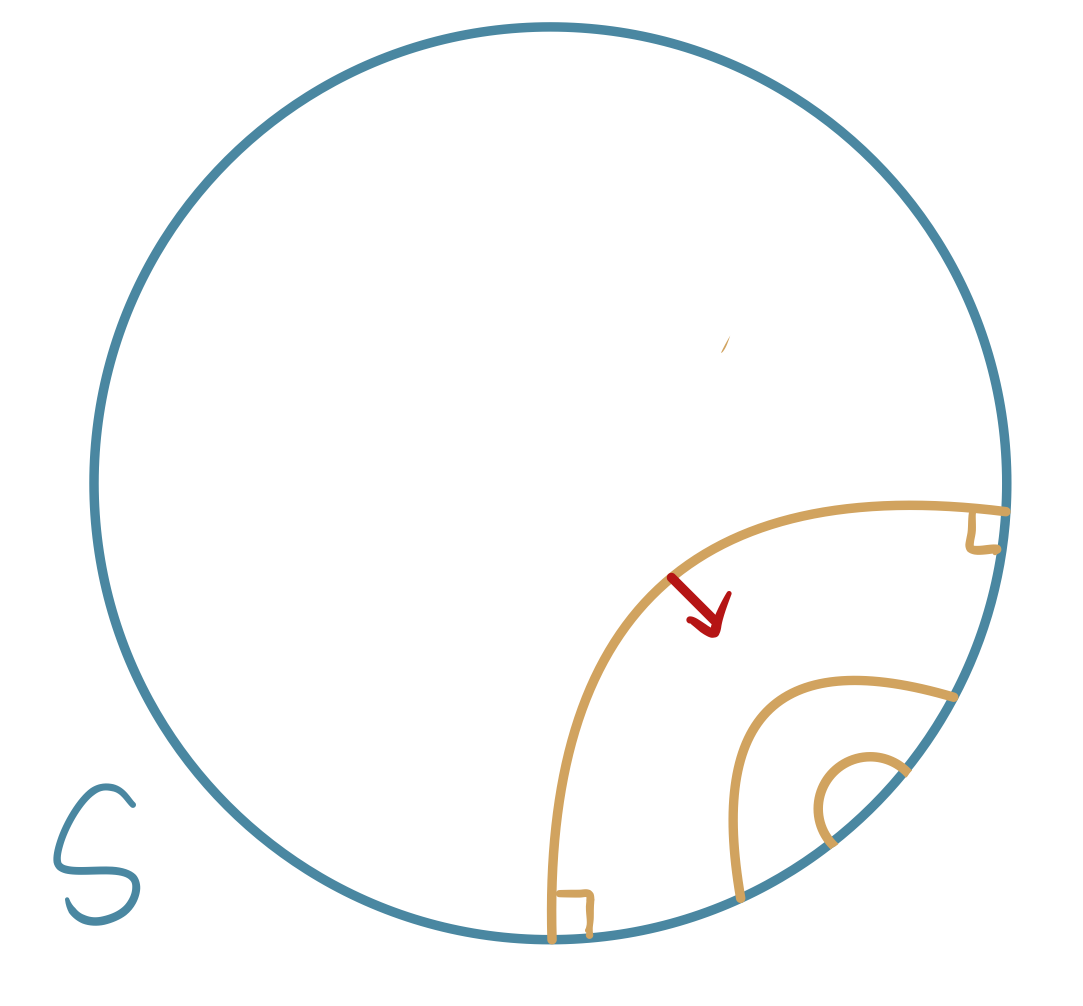
\includegraphics[scale=0.12]{StCon.png}
            \end{figure}
                
                
                \end{column}
            \end{columns}

        
    \end{frame}

    \begin{frame}
        \frametitle{General Strategies for Proving Convergence}
        
        \begin{enumerate}
            \item \textcolor{blue}{Preservation of convexity}\\
            Show that inequalities
            \[h_{ij}^{} \geq 0 \text{ and }\epsilon H g_{ij }^{} \leq h_{ij }^{} \leq \beta H g_{ij }^{} \]
            are preserved under the flow.
            \item \textcolor{blue}{Pinching estimate}\\
            Show that the quantity
            \[\left| A \right| ^2-\frac{1}{n}H^2=\frac{1}{n}\sum_{i<j}^{n}(\kappa _i-\kappa _j)^2\]
            which measures the sum of differences between eigenvalues $\kappa _i$ of the second fundamental form $A$ is relatively small.
        \end{enumerate}
        
    \end{frame}

    \begin{frame}
        \frametitle{Main Results}
        In this thesis, we focus on mean curvature flow with free boundary in an ambient Riemannian manifold $\bar{M}$ and obtain the following two results:
        \vspace{0.4cm}
        \begin{itemize}
            \justifying
            \item computation of the boundary derivative of the second fundamental form
             \vspace{0.2cm}
            \item establishment of an iteration scheme for obtaining uniform bounds of functions on hypersurfaces under the flow.
        \end{itemize}
    \end{frame}

    \begin{frame}
        \frametitle{Boundary Derivatives}
        Instead of choosing a \textbf{coordinate system} to simplify computations, we work with the \textbf{tangent and normal bundles} over the space-time domain $\Sigma \times [0,T)$ and compute \textcolor{blue}{boundary derivatives} of the second fundamental form.
        \begin{theorem}
            Let $p \in \partial \Sigma$. For $u,v \in T_p \partial \Sigma $, 
    \begin{equation*}
        \begin{split}
            \nabla _N h(u,v)
            =& \left( \nabla _{F_*u}A^S(\iota \nu , F_*v)+A^S(\bar{\nabla }^{S}_{F_*u} \iota \nu , F_*v)  \right)   \nu \\
            & +A^S(F_*u, F_* v)h(N,N)-h(\nabla_u N, v) \\
            & + A^S(\iota  \nu  , \iota \nu )h(u,v) +\textcolor{red}{\overset{\perp }{\pi} (F^*R_{\nabla }(u,N)(F_* v))}.
    \end{split}
    \end{equation*}
        \end{theorem}
    \end{frame}

    \begin{frame}
        \frametitle{Stampacchia's Iteration}
        We prove that if a function on the hypersurface evolving under MCF satisfies two special inequalities, then this function is uniformly bounded in spacetime.\\
        \vspace{0.2cm} 
        Most of the arguments are similar to the proof of \textbf{Edelen(2016)} where the major difference is the establishment of a \textcolor{blue}{Michael--Simon type inequality} for free-boundary Riemannian submanifolds using a Sobolev type inequality proved by \textbf{Hoffman-Spruck(1974)}.
        \begin{theorem}
            For any $\Sigma $ meeting $S$ orthogonally, any $f \in C^{1}(\bar{\Sigma })$ with \textcolor{red}{$\left| \text{supp } f \right| $ sufficiently small}, and any positive integer $p<n$, there exists a constant $c=c(n,p,S,\bar{M})$ such that 
            \[\left\| f \right\| _{\frac{np}{n-p};\Sigma } \leq c(\left\| \nabla f \right\| _{p;\Sigma }+\left\| Hf \right\| _{p;\Sigma }+\left\|  f \right\| _{p;\Sigma }).\] 
        \end{theorem}
    \end{frame}

    \begin{frame}
        \frametitle{Future Directions---Convergence Theory}
        \begin{itemize}
            \justifying
            \item Using boundary derivatives, we will show the preservation of convexity and curvature pinching. When the barrier surface is not umbilic, cross terms that are uncontrollable by lower order terms will appear in the boundary derivatives.  To cancel problematic cross terms, one could do a perturbation to the second fundamental form, c.f. \textbf{Hirsch-Li(2020)}, \textbf{Edelen(2016)}, \textbf{Huisken-Sinestrari(1999)}.
            \item Using Stampacchia's iteration, we will show that \[f_\sigma =  \frac{\left| A \right| ^2-\frac{1}{n}H^2 }{H^{2-\sigma}} \] is uniformly bounded and derive the gradient estimate \[\left| \nabla H \right| ^2 \leq \eta H^4 + C\] to compare the mean curvature at different points.
        \end{itemize}
    \end{frame}

    \begin{frame}
        \frametitle{Future Directions---Higher Codimension}
        
        Applying the covariant formulation, \textbf{Andrews-Baker(2010)} proved a convergence theorem for higher-codimension submanifolds in $\R^n$ .

        We are interested in generalizing the above result to the free boundary case. We need to formulate the question carefully depending on the dimension of barrier surfaces.

        \begin{figure}[h]
            \centering
            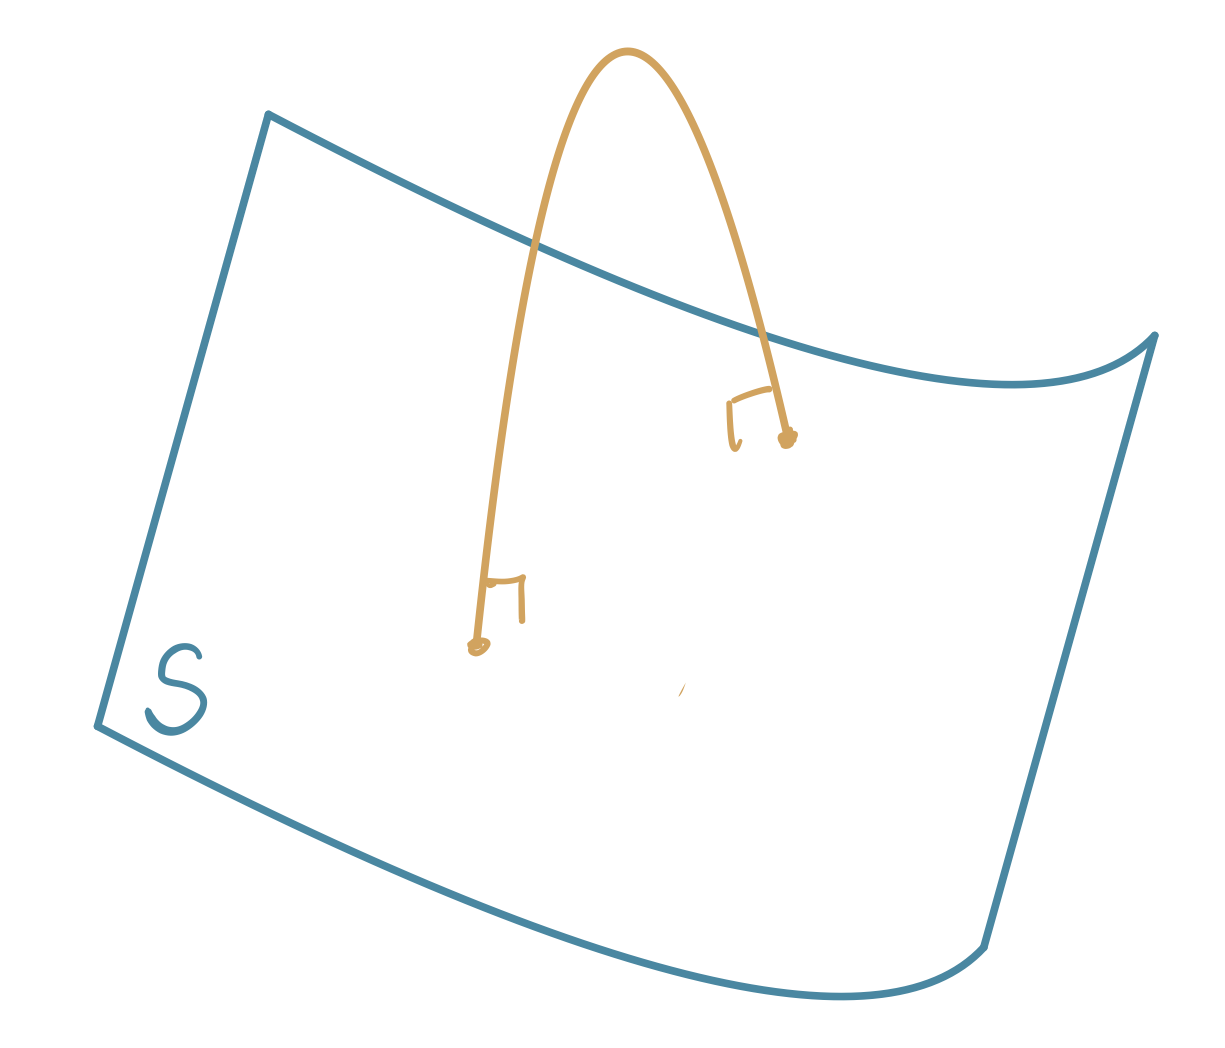
\includegraphics[scale=0.12]{HiCo.png}
            \caption{A higher-codimension surface with free boundary}
        \end{figure}
    \end{frame}

    \begin{frame}
        \centering \Large
        Thank you!
    \end{frame}


\end{document}